\documentclass[10pt]{article}
%% The amssymb package provides various useful mathematical symbols
\usepackage{verbatim}
\usepackage{amssymb}
\usepackage{subfigure}
\usepackage{epsfig}
\usepackage{psfrag}
\usepackage{ulem}
\usepackage{multirow}
\usepackage{booktabs} %for table in the form Excel2Latex
\usepackage{bm} %bold greek letter.
\newtheorem{theorem}{Theorem}
\newtheorem{remark}[theorem]{Remark}

\newcommand{\rd}{\mathrm{d}}
\newcommand{\be}{\begin{eqnarray}}
\newcommand{\ee}{\end{eqnarray}}
\usepackage{tabularx}% http://ctan.org/pkg/tabularx
\renewcommand{\arraystretch}{1.5} % tables have longer cells
%\journal{Undecided Journal}

\begin{document}
\section{An evolutionary game theory model for devaluing rhinos}
19 April 2017

\subsection{Introduction}
The illegal trade in rhino horn supports aggressive poaching
syndicates and a black market (Nowell et al., 1992). This lucrative market entices people to invest their time and energy to gain a `winfall' in the form of a rhino horn, through the poaching of rhinos. In recent years poaching has escalated to an unpresidented level resulting in concerns over their future existence (Smith et al., 2013). In response, rhino conservation has seen increased militarisation with `boots on the ground' and `eyes in the sky' (Duffy et al., 2015). An alternative method is to devalue the horn itself, one of the main methods being the removal so that only a stub is left. The first attempt at large-scale rhino dehorning as an anti-poaching measure was in Damordond, Namibia, in 1989 (Milner-Gulland and Leader-Williams, 1992). Other methods of devaluing the horn that have been suggested include the insertion of poisons, dyes or GPS trackers (Gill, 2010; Smith, 2013). However, like dehorning, they cannot remove all the potential gain from an intact horn (poison and dyes fade or GPS trackers can be removed). This paper considers the general strategy of devaluing horns, which includes dehorning.

Rhino populations now persist largely in protected areas or
on private land, and require intensive protection (Ferreira et al., 2014). For wildlife managers law enforcement is often one of the main methods of deterring poaching, however rhino managers can remove the poaching incentive by devaluing their rhinos (MilnerGulland, 1999).

A manager does not need to choose law enforcement or devaluing, but perhaps adopt a combination of the two; especially given that devaluing rhinos comes at a cost to the manager, and the process comes with a risk to the rhinos. Milner-Gulland and Leader-Williams (1992) found the optimum proportion to dehorn using mean horn length as a measure of the proportion of rhinos dehorned. They showed, with realistic parameter values, that the optimal strategy is to dehorn as many rhinos as possible.

A recent paper modelled the interaction between a rhino manager and poachers using game theory (Lee et al. 2016). The authors consider one year only, for a single rhino manager. They assume a given amount of resource available for the year, and that all rhinos initially have intact horns. Rhino managers may devalue a proportion of their rhinos. The manager intends to devalue as few as possible, whilst still ensuring the safety of their rhinos. The remainder of his/her resources is spent on security. Poachers may either only kill rhinos with full horns, `selective poachers', or kill all rhinos they encounter, `indiscriminate poachers'. If all rhinos are left by the rhino manager with their intact horns, it does not pay poachers to be selective so they will become indiscriminate poachers.
Conversely, if all poachers are selective, it pays rhino managers to invest in devaluing his/her rhinos. This dynamic is represented in Fig.~\ref{fig:RhinoPic}. Assuming poachers and managers will always behave so as to maximise their payoff, there are two equilibriums: either all devalued and all poachers selective; or all horns intact and all poachers indiscriminate. Essentially, either the managers win, the top left quadrant
of Fig.~\ref{fig:RhinoPic}, or the poachers win, the bottom right quadrant of Fig.~\ref{fig:RhinoPic}. The paper concludes that poachers will always choose to behave indiscriminately, and thus the game settles to the top left quadrant, i.e., the poachers win. 

We develop upon this model further using evolutionary game theory. This means that the preferred strategy of a poacher may change as the system evolves. For example, as the quantity of rhino horn gained increases, standard supply and demand arguments indicate that the value of the rhino horn decreases (REF). Therefore, this model allows for interaction between poachers over multiple plays of the game. 

The players are no longer the rhino manager and rhino poachers, but poacher versus poacher. The rhino manager creates the conditions in which they play. The purpose is to discover the conditions which best encourages the poachers to behave selectively, that is, they only kill those rhinos with full horns. 
\begin{figure}
\centering
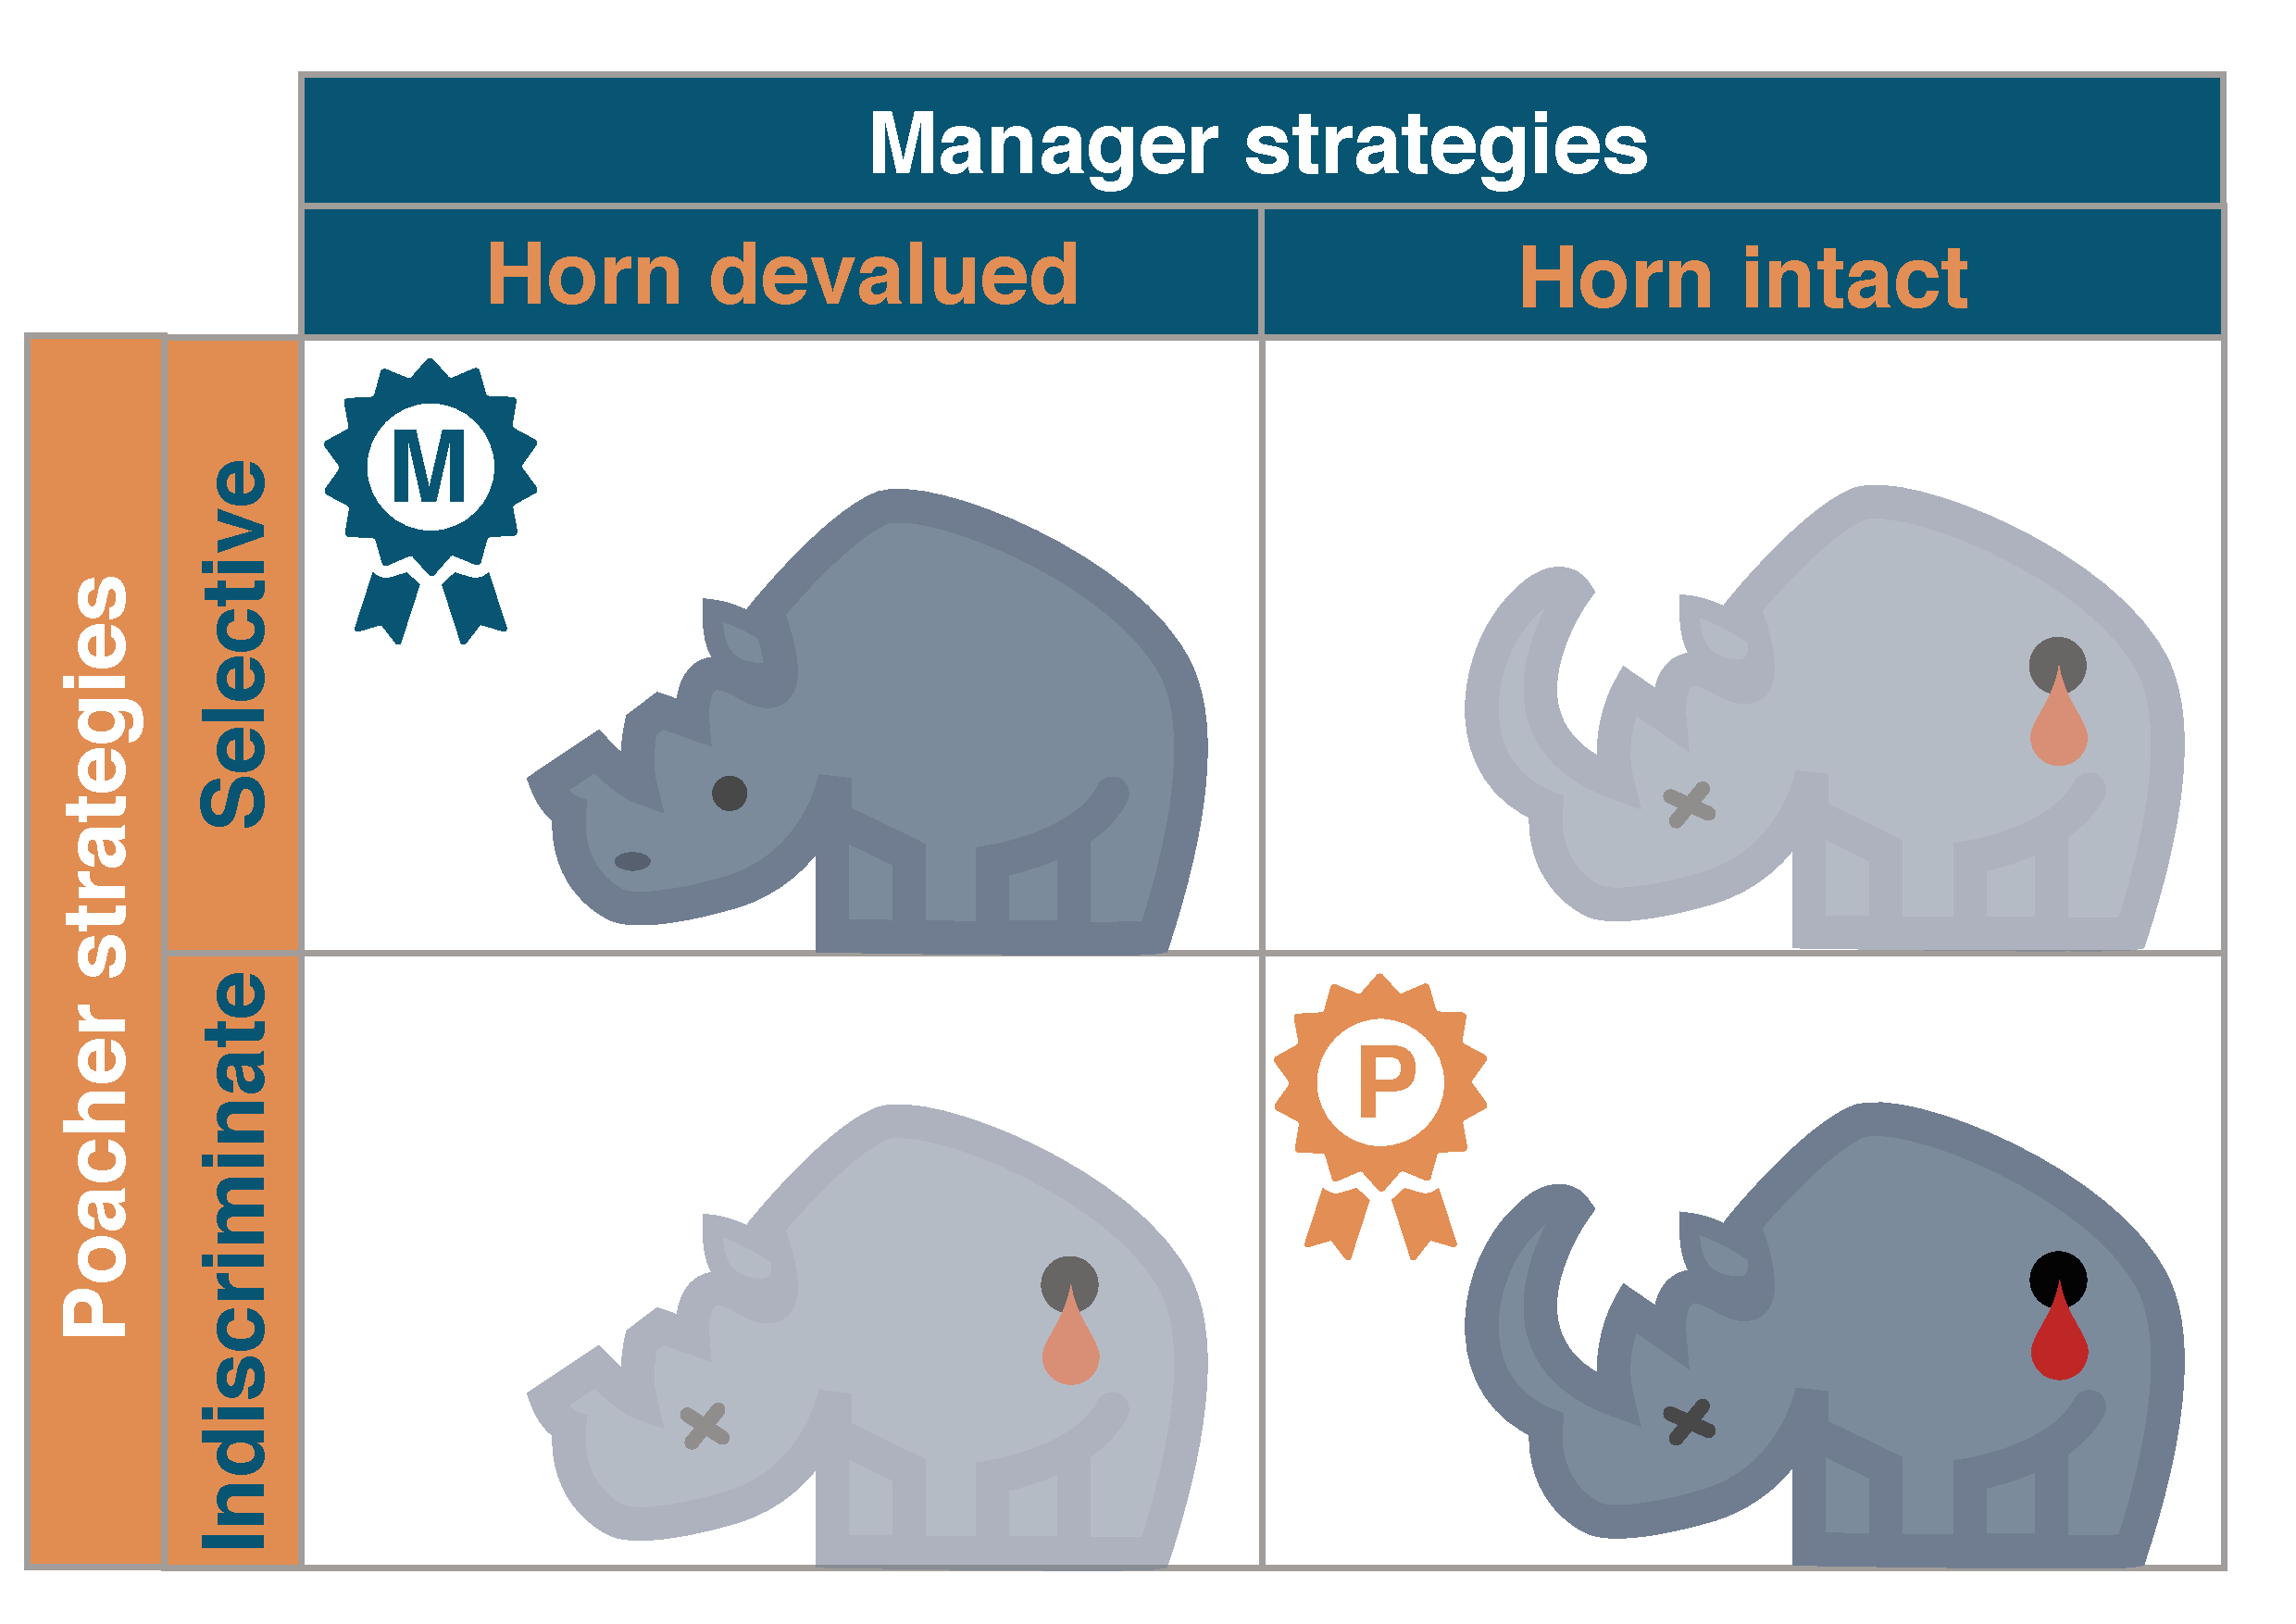
\includegraphics[scale=0.2]{RhinoPic.pdf}
\caption{\label{fig:RhinoPic} The game between rhino manager and rhino poachers. The system settles to one of two equilibriums, either devaluing is effective or not. }
\end{figure}
\subsection{Method}

The poacher incurs a loss from seeking a rhino, and the risk involved. The gain depends upon the value of horn, the proportion of horn remaining after the manager has devalued the rhino horn and the number of rhinos (devalued and not). 

Let us first consider the gain to the poacher, where $\theta$ is the amount of horn taken. We assume rhino horn value is determined by weight only, a reasonable assumption as rhino horn is sold in a grounded form (savetherhino.org). Referring to Fig.~\ref{fig:RhinoPic}, clearly if the horn is intact, the amount of horn gained is $\theta=1$ for both the selective and the indiscriminate poacher. If the rhino horn has been devalued, and the poacher is selective, the amount of horn gained is $\theta=0$ as the poacher does not kill. However, if the poacher is behaving indiscriminately, the amount of horn gained is $\theta = \theta_r$. Therefore, assuming a linear relationship, the amount of horn gained in the general case is 
\begin{eqnarray}
\label{eqn:theta}
\theta(r,s) = s(1-r) + (1-s)((\theta_r -1)r + 1),
\end{eqnarray}
where $r$ is the proportion of rhinos that have been devalued, and $s$ is the proportion of selective poachers. Standard supply and demand arguments imply that the value of rhino horn decreases as the quantity of horn increases. Thus at any given time the expected gain for a poacher is 
\begin{eqnarray}
\label{eqn:world_gain}
H \theta(r,s)^{-\alpha},
\end{eqnarray}
where $H$ is a constant associated with the value of a full horn, and $ \alpha \geq 0$ is a constant that determines the precise relationship between the quantity and value of the horn. Thus, when a given individual interacts in the `world', the gain is either 
\begin{eqnarray}
\label{eqn:gain}
\left\{
\begin{array}{cl}
\theta(r,1) H \theta(s,r)^{-\alpha} & \mbox{ selective poacher}
\\
\theta(r,0) H \theta(s,r)^{-\alpha} & \mbox{ indiscriminate poacher}
\end{array} \right.
\end{eqnarray}
depending on the chosen strategy of the individual. 

Secondly we consider the costs incurred by the poacher. We assume that the risk to the poacher is the inverse of the proportion of rhinos devalued $r$, since the rhino manager can spend more on security if the cost of devaluing is low. Additionally, since indiscriminate poachers kill more rhinos they incur a greater risk. Therefore, the cost due to risk for a given individual is
\begin{eqnarray}
\label{eqn:phi}
\phi(r,s) = R_1 s + R_2 (1-s),
\end{eqnarray}
where $R_1 < R_2$. Thus, when a given individual interacts in the `world', the cost incurred due to risk is
\begin{eqnarray}
\label{eqn:loss_risk}
\left\{
\begin{array}{cl}
\phi(r,1) (1-r)^{-\beta} & \mbox{ selective poacher}
\\
\phi(r,0) (1-r)^{-\beta} & \mbox{ indiscriminate poacher}
\end{array} \right.
\end{eqnarray}
where $\beta \geq 0$ is a constant that determines the precise relationship between the proportion of rhinos not devalued (resources saved) and the security on the grounds.

Another cost to the poacher is seeking out a rhino. The proportion of rhinos that are not killed is $rs$. Therefore, for a given individual, the cost of finding a rhino that to kill is 
\begin{eqnarray}
\label{eqn:psi}
\psi(r,s) = 1-rs.
\end{eqnarray} 
Thus, when a given individual interacts in the `world', the cost incurred due to risk is
\begin{eqnarray}
\label{eqn:loss_finding}
\left\{
\begin{array}{cl}
\psi(r,1) F(1-rs)^{-\gamma} & \mbox{ selective poacher}
\\
\psi(r,0) F(1-rs)^{-\gamma} & \mbox{ indiscriminate poacher}
\end{array} \right.
\end{eqnarray}
where $F$ and $\gamma \geq 0$ are constants that determine the precise relationship between the proportion of vulnerable rhinos and the probability of finding a rhino, such that $\gamma$ close to zero indicates very sparse rhinos. 

Let  $\sigma = (1,0)$ represent an individual poacher who is selective and $\sigma = (0,1)$ represent an individual poacher who is indiscriminate. Combining~(\ref{eqn:gain}), (\ref{eqn:loss_risk}) and (\ref{eqn:loss_finding}) gives the utility function for the individual poacher $\sigma$ in the population $\chi$, 
\begin{eqnarray}
\label{eqn:utility}
u(\sigma, \chi) = s u(S,\chi) +(1-s) u(\bar{S},\chi), 
\end{eqnarray}
where
\begin{eqnarray}
\label{eqn:USchi}
u(S,\chi) &=& \theta(r,1) H \theta(r,s)^{-\alpha}
- \phi(r,1) (1-r)^{-\beta} 
- \psi(r,1) F(1-rs)^{-\gamma} ,
\\
\label{eqn:UnotSchi}
u(\bar{S},\chi) &=& \theta(r,0) H \theta(r,s)^{-\alpha}
- \phi(r,0) (1-r)^{-\beta}
- \psi(r,0) F(1-rs)^{-\gamma}.
\end{eqnarray}
Substituting~(\ref{eqn:USchi}) and~(\ref{eqn:UnotSchi}) into~(\ref{eqn:utility}) gives
\begin{eqnarray}
\label{eqn:utility2}
u(\sigma, \chi) &=& 
H (\theta_r r(s+1)-r+1)g(r,s)^{-\alpha} \\ \nonumber &&
-
(sR_1 + (1-s)R_2)(1-r)^{-\beta} - F(1-rs)(1-rs){-\gamma},
\end{eqnarray}
where 
\begin{eqnarray}
\label{eqn:g}
g(r,s) = s(1-r)+(1-s)((\theta_r+1)r+1) = \theta_r r + r + 1 - s(\theta_r - 2r).
\end{eqnarray}
Note that since $\theta_r, r, s  \in [0,1]$, then $g(r,s)>0$.
\subsection{Stable strategies}
When a strategy is stable, the individual $\sigma$ is representative of the population $\chi$. There are three stable strategies. Firstly where everyone is selective, secondly where everyone is indiscriminate, and thirdly, where there is a mix $\sigma^* = (s^*,1-s^*)$. We now discuss three different $s^*$ and establish whether it is evolutionary stable. If it is evolutionary stable, then the utility function~(\ref{eqn:utility}) for $\sigma^*$ in a mutated population $\chi_\epsilon$ is greater than an alternative $\sigma$ in the same mutated population,
\begin{eqnarray}
\label{eqn:ees}
u(\sigma^*,\chi_\epsilon) > u(\sigma,\chi_\epsilon).
\end{eqnarray}
That is, for the system to be evolutionary stable, even when the population is mutated, it is beneficial for the poachers to return to the equilibrium behaviour $\sigma^* = (s^*,1-s^*)$. The right-hand side of~(\ref{eqn:ees}) is simply~(\ref{eqn:utility2}) where $s=s_\epsilon$ to represent a mutation of $s$.
\subsubsection{All poachers are selective}
Consider the case where all poachers are selective,  $\sigma^* = (1,0)$, meaning that the left-hand side of~(\ref{eqn:ees}) is 
\begin{eqnarray}
\label{eqn:1a}
u(\sigma^*,\chi_\epsilon) = H(1-r)g(r,s_\epsilon)-R_1(1-r)^{-\beta} - F(1-r)(1-rs_\epsilon)^{-\gamma}.
\end{eqnarray}
The conditions under (\ref{eqn:1a}) is greater than (\ref{eqn:utility2}) provides the conditions under which the system is evolutionary stable when all poachers are selective. This essentially provides the conditions under which the rhino manager can deter poachers. 
\begin{eqnarray}
u(\sigma^*,\chi_\epsilon) -u(\sigma,\chi_\epsilon) &=& 
-rHg(r,s)^{-\alpha} 
\\ \nonumber &&- (1-s_\epsilon)(R_1-R_2)(1-r)^{-\beta} 
\\ \nonumber
&&+ Fr (1-s_\epsilon) (1-rs_\epsilon)^{-\gamma}.
\end{eqnarray}
Now $rHg(r,s_\epsilon)^{-\alpha}$ is positive (see~(\ref{eqn:g})), and $(R_1-R_2)$ is negative. Therefore, the system is evolutionary stable when 
\begin{eqnarray}
\label{ees1}
rHg(r,s)^{-\alpha} < (1-s_\epsilon)(R_1-R_2)(1-r)^{-\beta} +Fr (1-s_\epsilon) (1-rs_\epsilon)^{-\gamma}.
\end{eqnarray}

\subsubsection{All poachers are indiscriminate}
Consider the case where all poachers are selective,  $\sigma^* = (0,1)$, meaning that the left-hand side of~(\ref{eqn:ees}) is 
\begin{eqnarray}
\label{eqn:2a}
u(\sigma^*,\chi_\epsilon) = H((\theta_r-1)r+1)g(r,s_\epsilon)-R_2(1-r)^{-\beta} - F(1-rs_\epsilon)^{-\gamma}.
\end{eqnarray}
The conditions under (\ref{eqn:2a}) is greater than (\ref{eqn:utility2}) provides the conditions under which the system is evolutionary stable when all poachers are indiscriminate. This essentially provides the conditions under which the rhino manager cannot deter poachers. 
\begin{eqnarray}
u(\sigma^*,\chi_\epsilon) -u(\sigma,\chi_\epsilon) &=& 
Hr(\theta_r -1)g(r,s_\epsilon)^{-\alpha} 
\\ \nonumber &&- s_\epsilon(R_2-R_1)(1-r)^{-\beta} 
\\ \nonumber
&&- Fr s_\epsilon (1-rs_\epsilon)^{-\gamma}.
\end{eqnarray}
Since $\theta_r, r, s_\epsilon \in [0,1]$, and $(R_2-R_1)$ is positive, the system is never evolutionary stable.
\begin{thebibliography}{00}
% http://ams.org/msnhtml/serials.pdf

\end{thebibliography}


\end{document}

%%
%% End of file `elsarticle-template-num.tex'.
